\chapter{Fundamentals and Related Work}
\label{chap:1}
%
\section{State of the Art}

The most studies related to movement prediction on vehicles focus on lane change predictions. And there are various different methods are proposed to solve this task, the most popular are: \gls{DBN}, \gls{BN}, \gls{SVM}, \gls{HMM}, Mind-tracing and \gls{FL}. \\

\gls{BN} could be considered as a graphical representation of probability distribution. In \cite{BN1, BN2} \gls{DBN} and \gls{BN} are used to recognize actions which driver is intend to perform. Lateral movement of a vehicle is expressed using \gls{BN}, having several various nodes for probability. The probability distribution for every node is determined by doing an analysis of driver behaviour in the past while driving. And ultimately, the final prediction is obtained by calculating the probability of a certain movement with respect to the possibility for every node. \\

In \cite{Markov1, Markov2} process of driving is described as a set of various different states while driving. When some particular actions appear in particular defined sequence, it is possible to calculate the probability that the state will change to a particular state. In these works likelihood of states shifting is designed using \gls{HMM}. Authors of \cite{Markov3, Markov4} expanded their past work using even more realistic test case - they equipped a vehicle with sensors and used received graphical data to get more accurate results. Graphical models together with \glspl{HMM}  and its extensions were trained using the data from experimental driving,  seven different driver models were created: passing, changing lanes (to the right or to the left), turning right or left, starting and stopping. The result authors received and presented was "on average, the predictive power of our models is of 1 second before the maneuver starts taking place" \cite{Markov4}. \\

Author of \cite{Mind} proposed new method for prediction making, which was named Mind-tracing. It is a computational framework which is able to predict possible drivers' intentions. This method is different from others because here different cognitive model versions which include a flood of a possible intention and action is used. Each action and possible intention are compared with a driver's behaviour at the same time. And the closet to the human behaviours is used for the further intentions expression. \\

\cite{Fuzz} introduces \gls{FL} as an alternative method for modelling behaviour of the driver. The research paper is mainly focused on the process of decision making on lanes of a highway. For getting results a triangular membership function was used, fuzzy rules were defined by observing training procedure and learning from obtained results. The model was developed using actual traffic data. The used model combines the speed and speed difference of the vehicle, the lead and lag gap distances and the remaining distance to the end of the merge lane as input variables. The precision of prediction using the model was
higher than using the binary Logit model. The high prediction accuracy received using this model results in prediction accuracy made using this model overall. \\

\cite{VectMash} tested the validity and  accuracy of \gls{SVM} in movement prediction. After choosing proper hints for movement changing, data recorded by doing test were divided into different groups which were used for training classifier. Predictions were made using current information of the vehicle and classification hints at the current time. \\

Even though all methods have the same purpose, it is very hard to compare them directly. Results received having measurements in different situations and in different time steps, e.g. one research paper gives prediction two seconds in advance before a lateral position of vehicle’s overlaps with the lane border, while other paper gives prediction only one second before crossing the lane. Furthermore, there is no exact definition of \textit{lane crossing} moment, usually, it is the moment when vehicle cross edge of a lane, but in some paper, it is not clear enough. \\

Since it is not possible to make a clear comparison between methods due to essential differences in testing environments and different data sets, the Table \ref{table:DA} lists the best timing accuracy for each method. \\


\begin{table}[h]
	\caption{Different Methods Performance Comparison} 
	\centering 
	\scalebox{0.65}{
		\begin{tabular}{||c| c |c |c |c||}
			\hline\hline 
			\textbf{Method} & \textbf{References} & \textbf{Accuracy} & \textbf{Time}\\ [0.ex] 
			\hline\hline
			
			\textbf{(Dynamic) Bayesian Network} & \cite{BN1} & $80$\% & $1.5$s before changing movement \\
			& \cite{BN2} & 89\% & $0.5$s after changing movement \\ \hline   
			
			\textbf{Support Vector Machine}  & \cite{VectMash} & $87$\% & $0.3$s after changing movement  \\ \hline 
			
			\textbf{Hidden Markov Model}  & \cite{Markov1} & $89.4$\% & $2$s after changing movement \\ 
			& \cite{Markov2} & $95.2$\% & $2$s after changing movement \\
			& \cite{Markov3, Markov4} & Unknown & $0.4$s before any sign of changing movement appears \\ \hline 
			
			\textbf{Mind-tracing}  & \cite{Mind} & $82$\% & $1.1$s before changing movement \\ \hline 
			\textbf{Fuzzy Logic}  & \cite{Fuzz} & $86.8$\% & Unknown \\[1ex] 
			\hline  \hline
		\end{tabular}}
		\label{table:DA}
	\end{table}


As it is possible from the results shown in the table the best methods for predicting movement changes is received by using \gls{BN} and \gls{SVM}. These two methods are able to predict quite accurate and with a relatively short period of time, what will lead in having more time in advance to decide which action to make. \\

For further work, any Bayesian filter/classifier could be an acceptable method for examining behaviour of the driver for various reasons: 

\begin{itemize}
	\item Bayesian-based methods can perform well while working with a very big amount of data;
	\item It gives results with high accuracy from a problem, containing many features. It is needful to include different physical data while modeling and examining drivers’ behaviour. Traditional statistical classifiers most likely to be insufficient while processing high dimensional data.
	\item Bayesian filter/classifier are robust to over-fitting problem and rely on margin maximization instead of finding an edge for prediction directly from the training data.
\end{itemize}

\section{Probabilistic Estimation Methods}

Reasonable prediction and following decision-making process require considering uncertainty and objectives for the current situation. In this section, uncertainty will be represented as a probability distribution. \\

Uncertainty can be a result of partial information about the state of the world. In a real world trying to fulfil any given task, it is possible to meet various reasons which do not allow to finish a task without any difficulties. What means, that with information we have at hand, it is hardly possible to make a task evaluation with being completely certain. \\

Uncertainty can appear from practical and theoretical limitations while trying to predict future events, e.g., trying to exactly predict how a human would react in one situation or another, a decision support system would need to consider a model of the human brain. Even if the operation is known very well, it is still difficult to predict the end state and next actions which will be taken, due to spontaneous failures or other agent actions. \\

A robust prediction (and later decision) making system need to take into account sources of uncertainty, which exist in the current state and consider it when computing the future outcomes for events. In order to describe uncertainty
computationally, it needs to have a formal representation. 

\subsection{Belief State and Probability}

Solving tasks which involve uncertainty, it is very important to be able to compare the credibility of different statements. For example, if belief for action E is stronger than our belief for action T, then E $\succ$ T. If E and T have the same degree of belief, then E $\sim$ T. \\

It is also beneficial to be able to compare beliefs about statements considering some given information, e.g., we can say that likelihood for action C may happen while E condition is happening is bigger than having T, then this expression would be written (E | C ) $\succ$ (T | C ). \\

In order to make particular assumptions about the relationships of the operators $\succ$, $\prec$ and $\sim$. The assumption of \textit{universal comparability} and \textit{transitivity} assumptions requires to hold the same mathematical rules. Both assumptions allow representing degrees of belief by a real-valued function \cite{BOOK}, i.e. probability function P can be expressed like that:
\[ P(A|C) > P(B|C) \iff (A|C) \succ (B|C) \]
\[P(A|C) = P(B|C) \iff (A|C) \sim (B|C). \]

If new assumptions about the probability P form, then P need to satisfy the main axioms of probability: 0 $\leqslant$ P (A | B ) $\leqslant$ 1. If we are sure that A action will happen when B action is given then P (A | B ) = 1. If A action will not happen when B action is given, then
P (A | B ) = 0. \\

Deep review about probability theory won't be provided in here, but this work relies on important probabilities properties. The first of them is a definition of \textit{contidion probability}:

\begin{equation}
P(A|B)=\frac{P(A,B)}{P(B)},
\end{equation}

where P(A, B) shows the probability of A and B both being true. \\

Another property which is important is the \textit{law of total probability}, which states that if $\beta$ is a set of "mutually exclusive and exhaustive propositions" \cite{BOOK}, then

\begin{equation}
P(A|C)=\displaystyle \sum_{B \epsilon \beta}{P(A|B,C)P(B|C)}
\end{equation}

Finally, the most important rule for further work comes from the definition of \textit{conditional probability}:

\begin{equation}
P(A|B)=\frac{P(B|A)P(A)}{P(B)}.
\end{equation}

This equation is known as \textbf{\textit{Bayes’ rule}}, and as mentioned earlier, it will be very important for the following work. \\

But still, after this short introduction, question what exactly belied state is, still exists. One option to answer this would be the most believable next state for an examined object, considering experience in the past, which is given. This idea can be sound and save the basis for predictions in some cases, but in general, this idea is not sufficient. Being able to operate efficiently the degree of uncertainty must be taken into account, e.g. if the main agent is confused what future state could be, it could be proper to ask directions, take a look into the map, search for reference point, etc. \\

Other options for belief computation would be using probability distributions over states of the world, which we have. In this case, distributions encode the subjective probability for the main agent and include information about the state of the world and give a basis for taking action under uncertainty we have.  Moreover, sufficient statistical information of action made in the past and initial belief state of the agent is comprised, i.e. computed belief state for the current agent’s state and additional information about its past observations and/or action made, would provide any further information about the current state of the world \cite{belief}. \\

\textbf{Computing belief states}\cite{belief}: \\

A belief \textit{b} is a probability distribution over state space $\mathscr{S}$, \textit{b(s)} is the probability set to world state \textit{s} by belief state \textit{b}. The axioms for belief state is the same as for probabilities: 0 $\leqslant$ b(s) $\leqslant$ 1, for all s $\epsilon$ $\mathscr{S}$ and $\sum_{s \epsilon \mathscr{S} } b(s) = 1.$ At every new step, new belief \textit{b'} must be  computed given old belief \textit{b}, an action \textit{a} and an observation \textit{o}. The new belief of an new state \textit{b'(s')} can be calculated using formula:

\begin{equation}
\begin{split}
b'(s') = & \displaystyle Pr(s'|o, a, b) \\ 
& = \displaystyle \frac{Pr(o|s', a, b) Pr(s'|a, b)}{Pr(o|a, b)} \\
& = \displaystyle \frac{Pr(o|s', a) \sum_{s \epsilon \mathscr{S}} Pr(s'|a, b, s) Pr(s|a, b)}{Pr(o|a, b)} \\
& = \displaystyle \frac{O(s', a, o) \sum_{s \epsilon \mathscr{S}} T(s, a, s') b(s)}{Pr(o|a, b) }
\end{split}
\end{equation}

The denominator of equation (2.4), Pr(o | a, b), can be interpreted as a normalizing factor, which is independent of next state s', which causes the sum of belief of all possible next states to 1. The state estimator function SE(b, a, o), which task is to update the belief state based on the \textit{a, o} and the previous \textit{b}, as its output gives new belief for new state \textit{b'}. \\

Please note, that this subsection and the computation of belief states description is taken directly from \gls{POMDP} steps description. In later work, belief update will act an important role, but it will be computed using different components. Detail description of belief computation related to this work will be provided in next chapters. \\

To have particular classifier is not enough for making accurate trajectory and movement predictions. Next chapter introduce with the most popular model for movement predictions.

\section{Movement Prediction}

Foresee future moments and trajectories for dynamical objects in traffic scenarios is vital in order to obviate risks which occur on the roads. Prediction despite of short or long term they are, must have sufficient time in advance to avoid traffic situations we, as traffic participants, don't want. In this section, relevant researches for trajectory and movement predictions are introduced. \\

There is numerous research made on a trajectory and movement predictions with a vehicle as interest on traffic scenarios. \cite{ClassificationI} suggesting a one way of classifying methods for motion prediction. The main three categories with an increased rate of flexibility were defined: \textbf{\textit{physical-based, maneuver-based}} and \textbf{\textit{interaction aware}}.

\begin{itemize}
	\item \textbf{Physics-based} motion models are the most simple of all categories. It is considered that the movement of vehicles depends only on the laws of physics. A wider description is in subsection ~\ref{subsection:phb}.
	\item \textbf{Maneuver-based} motion models are more advanced than physics-based because maneuver-based motion models also consider future movements of a car which also depends on the maneuver which is intended to perform by a driver. A wider description is in subsection ~\ref{subsection:mb}.
	\item \textbf{Interaction-aware} motion models take into account consideration connections between maneuvers of the car, as well as rules of the traffic. This method as not so popular as previous ones due its complicity to adapt to the real life scenarios. A wider description is in subsection ~\ref{subsection:inaw}.
\end{itemize}

Figure~\ref{fig:MotModOv} summarizes motion models defined in \cite{ClassificationI}.

\begin{figure}[h]
	\centering  	
	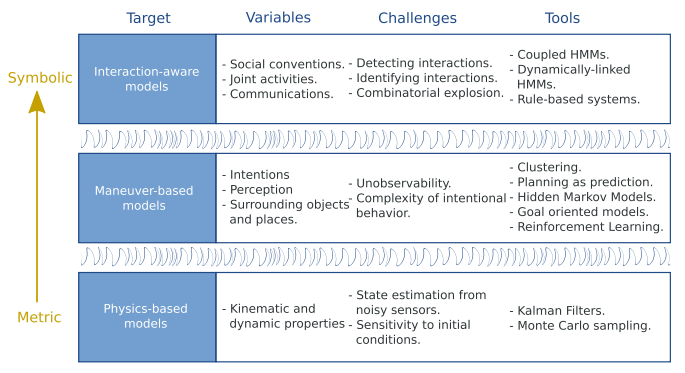
\includegraphics[width=13cm]{img/2.jpg}
	\caption{Motion Modeling Overview \cite{ClassificationI}}
	\label{fig:MotModOv}    
\end{figure}


\begin{figure}[h]
	\centering  	
	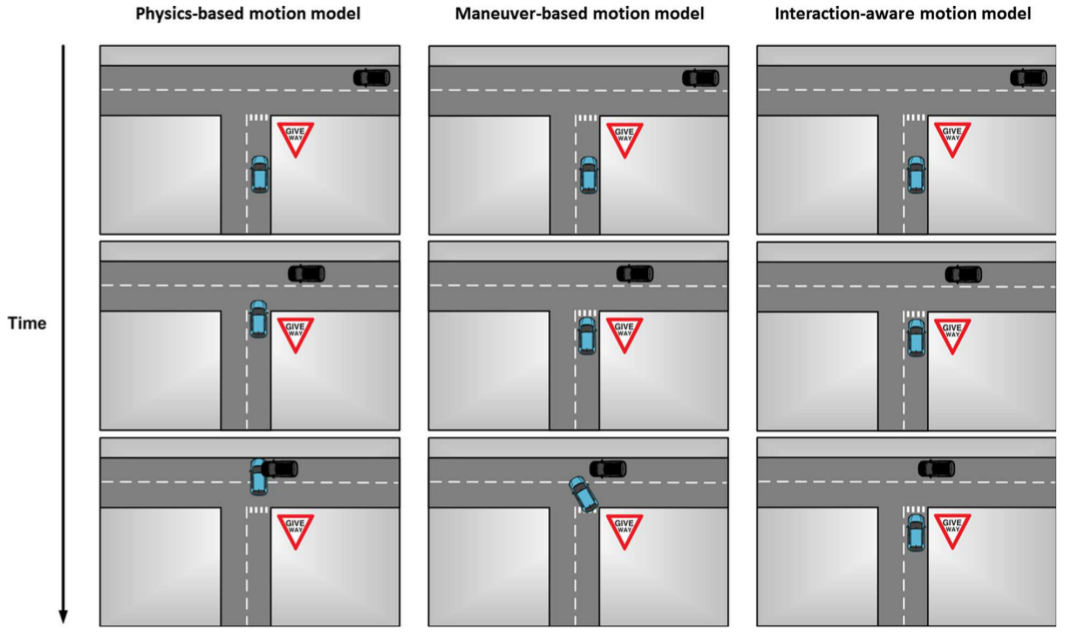
\includegraphics[width=13cm]{img/5.jpg}
	\caption{Examples of motion prediction with the different types of motion models \cite{ClassificationI}}
	\label{fig:MotModOv2}    
\end{figure}

Together with above-mentioned categories, authors of \cite{ClassificationII} introduced one more category to predict movements - \textbf{\textit{data-driven based}}.

\begin{itemize}
	\item \textbf{Data-driven} based motion and trajectory prediction can be classified into clustering-based and probabilistic approaches. A wider description is in subsection ~\ref{subsection:ddr}.
\end{itemize}

\subsection{Movement Prediction Using Physics-Based Models}
\label{subsection:phb}

Physics-based movement prediction models imply vehicles as a dynamic item, controlled by the physics' laws. Movements are predicted using dynamic and kinematic models with control inputs (e.g. acceleration, deceleration, steering), properties of the car (e.g. length, weight) and some external conditions (e.g. the friction coefficient of the road surface) to the process state of the vehicle (e.g. position, speed, direction). Great work has been done using \textit{physics-based} motion models and it still remains the most commonly used motion models for motion prediction in the context of road safety. The complexity of the models depends on a representation of the dynamics and kinematics of a vehicle, as well as, how uncertainties are handled, whether or not the road geometry is taken into account, etc. \\

Dynamic and kinematic models can be used for movement prediction in a lot of different ways, the main difference is how uncertainties are handled. Three main approaches will be described as follow: \textbf{\textit{single trajectory simulation, Gaussian noise simulation}} and \textbf{\textit{Monte Carlo simulation}} \cite{ClassificationI}.

\begin{itemize}
	\item \textbf{Single Trajectory Simulation.} The simplest method to predict future movements and trajectory of a car is to apply simple dynamic or/and kinematic models for the current state of a car while assuming that the current state of the car is determined with absolutely highest confidence and applied model (dynamic, kinematic or both) is the perfect representation for the movement of the car. This simple approach was used in \cite{dynamic} using dynamic and \cite{kinematicI, kinematicII} kinematic models. The main benefit of this straightforward approach is computational efficiency, that allows this method to be used in real time. On the other hand, predictions made by this method do not consider uncertainties of the current state and as a result, predicted movements and trajectories are not trustworthy for use in a long term ( > 1 sec.) predictions.
	\item \textbf{Gaussian Noise Simulation.} The uncertainty of the current state of a vehicle and its evolution during the time is a very important factor in movement or trajectory prediction and it can't be avoided. In \cite{GaussianNoiseI, GaussianNoiseII, kinematicII} this is modelled using a normal distribution. Gaussian Noise function is very popular because of its uncertainty representation in \gls{KF}, which is still a conventional method for vehicle state estimation having noisy sensors measurements in account. There are some cases where dynamic, kinematic and sensor models are linear and uncertainty is modelled using a normal distribution instead of \gls{KF} Bayesian filter is used. Filtering mainly contains of two steps: prediction and update steps. In the first time step at time step t, a current state of the vehicle is is given to the dynamic or kinematic model, which gives predicted state for the next time step which has a Gaussian distribution shape. In the following step, predicted state of the next time step is combined with sensor measurements of the same time step, which is Gaussian distribution as well. Filtering is a looping of these two steps every time when new measurements are available.
	
	By looping the first step, it is possible to get a mean and covariance matrix for every future timestep for the vehicle state. This can be modified into a trajectory mean with linked uncertainty (i.e. normal distribution in each timestep), as showed in \cite{GaussianNoiseIII, GaussianNoiseI}. As compared to the approached of \textit{single trajectory simulation}, Gaussian Noise simulation techniques have the benefit of uncertainty representation on the predicted trajectory or movements. However, there are some limitaitons as well: modelling uncertainties employing normal distribution is not quite enough to show the different possible maneuvers. A possible solution for this could be uncertainty representation using \gls{VGMM}. Author of \cite{SKFI} used \gls{SKF} for this exact purpose. \cite{GaussianNoiseII} depends on mass of \gls{KF} to show possible models for movement evolution for vehicle and be able to freely change between them. \cite{kinematicII} introduced an alternative approach: to use heuristics and change different kinematic model depending on the current situation.
	
	\item \textbf{Monte Carlo Simulation.} In generic case  when no assumptions in advance are made about models linearity or uncertainty model, distribution expresion on predicted vehicle states are not clear. Monte Carlo method is the right tool for this kind of situation. The idea under the Monte Carlo method is to randomly sample the input of the dynamic or kinematic model and to generate potential future trajectories. If the road topology is taken into account, various mass can be added to the generated trajectories and movements to penalize the ones which do not respect the restriction of the road design. Kinematic and dynamic models can be used for Monte Carlo method by categorizing inputs instead of considering them as a constant. Typical inputs are categorized to acceleration, steering angle or lateral deviation. To be able to take into account eligibility of the movement, generated trajectory samples, which has a bigger acceleration than physically is allowed can be removed, as it was done in \cite{MonteCarlo} or consider limitations which vehicle has (weight, length, etc.) and distribute dynamic and kinematic models in a more realistic manner and remove all impracticable trajectories from predefined trajectories list as it was done in \cite{MonteCarloI}. Monte Carlo method can be used to foresee trajectory or movements for a vehicle with a very well known current state or for vehicle which has uncertainty in the current state, which was estimated by one of the filtering algorithms.
\end{itemize}

\subsection{Movement Prediction Using Maneuver-Based Models}
\label{subsection:mb}

\textit{Maneuver-based} motion models show vehicles as independent moving entities, i.e. it is assumed that the movement of a vehicle on the road match to a series of independently executed movements from the other vehicles on the same road. Oxford dictionary \cite{def} a movement/maneuver as “a physical movement or series of moves requiring skill and care”. Term behaviour in literature often is used meaning the same meaning, e.g. in \cite{beh1, beh2, beh3}, for the sake of simplicity word "movement" or "maneuver" will be used in this work with defined meaning. Movement and trajectory prediction using maneuver-based motion models work with in advance recognized movements which driver possibly intend to perform. If an algorithm can recognize intended movement, the algorithm can assume that future actions of the driver will match the recognized movement. Due to this a \textit{priori} information, trajectories received with this method are more relevant and reliable than the ones received using physics-based motion models.  Maneuver-based motion models rely on prototype trajectories or on movement intention estimation. \\

Vehicle motion classification into maneuver/movement classes has been extremely widely applied not only in driver assistance systems but into natural driving studies \cite{DataDrivenIV, DataDrivenV, DataDrivenVI, mab1, mab2, mab3, mab4, mab5, mab6, mab7}. Authors of the majority of approaches are using heuristinc \cite{mab1} or training classifiers like \glspl{SVM} in \cite{mab2}, \glspl{HMM} \cite{DataDrivenIV, mab3, mab4}. \glspl{LSTM} in \cite{mab5}, Bayesian networks \cite{mab6}, etc., as movement-based features using speed, deceleration, acceleration, yaw rate, lane position, turn signals, distance from other vehicle and other road context information. Authors of \cite{mab1} classified vehicle's movement into class "keep lane" or "change lane" grounded on how far the closest car is and predicted future trajectory by applying quintic polynomial of the current car movement state and pre-defined ultimate movement state for each movement class, defined before.Authors of \cite{mab6} used six different movement classes, which were defined before and using \gls{DBN} based on multiple movements and context based features selected the potentially right future movement. Authors of \cite{mab7} defined an individual Gaussian process for three movement classes and established a multi-modal distribution for possible future trajectories using each model. However, in the study, only one case-based prediction has been introduced. Authors of \cite{DataDrivenIV} also determined separate Gaussian processes, this time for four different movement classes, which were classified using a hierarchical \gls{HMM}. This method was tested on real highway data. Authors of another study \cite{DataDrivenV} used a random forest classifier for movements classification into pre-defined movement classes: left or right lane changes or keep lane. Authors used a separate \gls{GMR} model for predicting lateral movement for vehicles using each class. Method was tested on real highway data. Similar method, but without predifined movements classes for prediction longitudinal motion for vehicles were used in \cite{DataDrivenVI}.

\subsection{Movement Prediction Using Intention Aware Models}
\label{subsection:inaw}

\textit{Interaction-aware} motion models introduce cars as
manoeuvring items which co-operate with each other, i.e. a movement of a vehicle is considered to be affected by a movement of the other moving object in the traffic scene. Keeping into account the dependencies between the separate moving objects leads to a much better explanation of their movement compared with \textbf{maneuver-based} motion models described in the previous subsection.  As a result, it gives a better perception of the current situation. \\

Despite this, a relatively small amount of researches is done considering inter-moving-objects interaction in movement prediction. Authors of \cite{InterAwareI} assigned two movement classes for vehicles approaching an intersection together, applying a polynomial classifier which "punishes" cases that potentially would lead to near-collisions situations. Authors of \cite{InterAwareII} worked with a much complex scenario and assigned movement classes to multiple together interacting vehicles in a highway scenario. However, foreseen movements, trajectories of a vehicle are assumed to be given in advance. Results reported using a simulated environment. \cite{ClassificationII} in their work considered multiple interacting vehicles together with the difficulty of estimating their future motion.  Authors of \cite{DataDrivenV} not directly used inter-moving-objects interaction by including comparative positions and velocities of vehicles close by as features for movement and trajectory prediction.

\subsection{Movement Prediction Using Data-Driven Model}
\label{subsection:ddr}

As mentioned earlier \textit{data-driven} movement prediction can be generally classified into clustering-based and probabilistic approaches.  \textbf{Clustering-based} approaches group the training data in order to provide a set of possible prototype trajectories \cite{DataDrivenI, DataDrivenII}. Partially observed trajectories are checked and compared with a prototype trajectory using various distance measurements, as \gls{DTW}, \gls{LCSS}, Hausdorff distance, etc. and after matching movement trajectory with prototype trajectory, later one is used as a model for future movement. Clustering approach is quite easy, but the main disadvantage of this method is the deterministic nature of the predictions. \\

\textbf{Probabilistic} approach contrary learn probability distribution of every movement trajectory class and gives the conditional distribution for future movements, given current trajectory. This lets us avoid some degree of natural uncertainty of predicting the future. \\

Authors of \cite{DataDrivenIII, DataDrivenIV} for modelling trajectories and for motion prediction use Gaussian Processes which are the most popular approaches solving prediction problems so far. \cite{DataDrivenV} uses \gls{GMR} for prediction longitudinal movement of a vehicle, while \cite{DataDrivenVI} uses the same method for lateral movement prediction. \cite{DataDrivenVII} uses \glspl{VGMM} for conditional distribution within snippets of future having snippets of movement history models. The latest approach is much easier and computationally more effective when compared to Gaussian Process Regression.  Authors proved the efficiency of method predicting non-linear movements in turns at the intersection scenarios. 

\subsection{Limitations of Methods for Movement Prediction}

Subsections~\ref{subsection:phb},~\ref{subsection:mb},~\ref{subsection:inaw} and~\ref{subsection:ddr} described movement prediction with different feature based model. This subsection will introduce limitations of all these methods.

\begin{itemize}
	\item \textbf{Physics-based approach.} Predictions using physics-based motion models are restricted to very short-term ( < $1$ sec.) motion prediction due to low-level motion (dynamic and kinematic) properties this method relies on. Usually using this method it is  unable to foresee any change in the vehicle movement which happens due to an execution of a particular maneuver (e.g. speed up, slow down, make a turn, etc.), or changes caused by external factors (e.g. slowing down due to traffic lights, signs, other vehicles, etc).
	
	\item \textbf{Maneuver-based approach.} For a very long time, the biggest limitation of prototype trajectories was time representation. When the movement models are showed using a finite set of trajectories it takes a very large number of prototypes to represent the large variation
	in the implementation of an every possible movement pattern. Handling subtle situation in traffic, as movements with waiting time at a stop line, not constant velocity caused by traffic is a very big issue for such models. For a certain extent, \gls{GP} were introduced. They solved this kind of problem by introducing time-independent movement patterns \cite{DataDrivenIII}. On the other hand, \glspl{GP} have some other limitations as well. First of all to be able to take into account all possible traffic scenarios, has very heavy computational time, despite that they are not considering the physical limitations of a vehicle and due to that may generate or predict unrealistic trajectories and movements. To solve these problems the best solution so far was proposed in \cite{RRT}. Authors used \gls{RRT} to be abe to "randomly sample points toward dynamically feasible trajectories, using as inputs the current state of the vehicle and the sample trajectories generated by the \glspl{GP}"  \cite{RRT}. Another issue with using predefined prototype trajectories is an adaptation to a different road, i.e. for different intersections. Each movement model is defined for a specific road/intersection geometry and topology, what means that prototype models only can be used with the same or very similar topology. 
	
	Maneuver-based approach contains similar limitations which described under limitations of data-driven approach.
	
	\item \textbf{Interaction-aware approach.} Prediction using interaction-aware motion models are the most exhaustive method suggested in the literature so far. Using it, is possible to predict for a longer-term as compared to physics-based motion prediction models, and predictions are more trustworthy than using maneuver-based motion models in predictions due to taking dependencies between the surrounding cars into consideration. However this completeness has some disadvantages as well:  calculation of all possible trajectories with all possible models take a lot of time and because of that, it is not very compatible with using in real-time situations. For this reason, using interaction-aware motion predictions are not so popular. 
	
	\item \textbf{Data-driven approach.} The assumption that movement of vehicles do not depend on each other and other traffic participants is not accurate.  All vehicles without any exceptions use a road together with other traffic participants and movement performed by one vehicle directly or indirectly effects others. Dependencies with each other are quite strong at intersection, where road rules, not only movement of other cars must be taken into account. Ignoring these reliances can lead to wrong interpretations of the situations, and affects the evaluation of the risk. A data-driven approach is quite easy, but not always it pays attention to these critical dependabilities and it is quite difficult to pre-define all possible action of other traffic participants, i.e. the main disadvantage of this method is the deterministic nature of the predictions.
\end{itemize}